\chapter{訓練環境}
\section{OpenAI Gym}
 Gym 是用於開發和比較強化學習算法的工具包,他不對agent的結構做任何假設,並且與任何數據計算庫兼容,而可以用來制定強化學習的算法。這個環境具有共享的介面,使我們能用來編寫常規算法,也就能教導agents如何步行到玩遊戲。\\[6pt]

\section{Pong}
 取自 1977年發行的一款家用遊戲機ATARI 2600中的遊戲,內建於Gym,這是一個橫向的乒乓遊戲,左方是預設電腦玩家,右邊由使用者或是由訓練程式控制(圖.\ref{fig.pong})。在強化學習範例中,Pong與實體冰球機簡化後環境相似。\\
\begin{figure}[hbt!]
\begin{center}
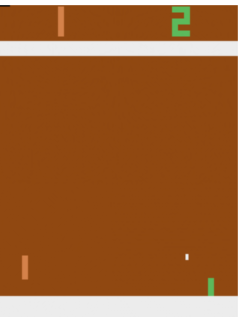
\includegraphics[height=8cm]{pong_gym}
\caption{\Large ATARI Pong}\label{fig.pong}
\end{center}
\end{figure} 

\newpage